\icode{E-MD-CA-L3-261120-004}
小明在学习道路交通安全时，了解到装载电线杆的货车由于刹车过急，导致装载的电线杆直接贯穿了驾驶室。为研究这类交通事故，小明同学建立了物理模型：水平车箱内叠放三根完全相同的圆柱体电线杆，其横截面如图所示；设每根电线杆的质量为 \(m\)，相邻电线杆间的动摩擦因数为 \(\mu\)，最大静摩擦力等于滑动摩擦力，电线杆前端与驾驶室间的距离为 \(d\)，货车以速度 \(v_0\) 在平直公路上行驶；若紧急刹车过程中货车做匀减速运动，下方的两根电线杆未分离且与车箱保持相对静止，重力加速度为 \(g\)。
	
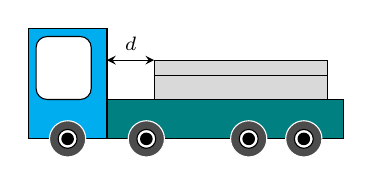
\begin{tikzpicture}[>=stealth,font=\scriptsize]
	\draw[fill=cyan] (0,0) rectangle(1,1.4);
    \draw[fill=teal] (1,0) rectangle(4,.5);
	\draw[rounded corners,fill=white] (.1,.5) rectangle(.8,1.3);
	\foreach \x in {.5,1.5,2.8,3.5}{
		\draw[white,fill=black!70] (\x,0) circle(.23);
		\draw[fill=white] (\x,0) circle(.12);
			\fill (\x,0) circle(.08);}
	\draw[fill=gray!30] (1.6,.5) rectangle(3.8,.8) (1.6,.8) rectangle(3.8,1);
	\draw[<->] (1,1)--node[above]{\(d\)}(1.6,1);
\end{tikzpicture}
\hspace{3em}
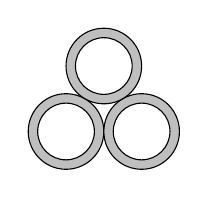
\begin{tikzpicture}[scale=.6]
	\coordinate (a) at(-.8,0);
	\coordinate (b) at(.8,0);
	\coordinate (c) at(0,{.8*sqrt(3)});
	\foreach \c in {a,b,c}{
		\draw[fill=gray!50] (\c) circle(.8);
		\draw[fill=white] (\c) circle(.6);}
\end{tikzpicture}
\begin{enumerate}
	\item 若货车制动距离为 \(s\)，制动时间为 \(t\)，且上、下电线杆间未发生相对滑动，求上方电线杆在此过程中所受摩擦力的合力大小；
	\item 若要保持上、下电线杆间不发生相对滑动，求货车刹车时的最大加速度大小；
	\item 若要使电线杆在刹车过程中不冲撞驾驶室，求货车的最小制动距离。
\end{enumerate}
\begin{answer}
	（1）\(\frac{2ms}{t^2}\)（2）\(\frac{2 \sqrt{3}}{3}\mu g\)（3）\(\frac{\sqrt{3} v^2}{4\mu g} - d\)
\end{answer}